%
% spielb.tex -- slide template
%
% (c) 2021 Prof Dr Andreas Müller, OST Ostschweizer Fachhochschule
%
\bgroup
\begin{frame}[t]
\setlength{\abovedisplayskip}{5pt}
\setlength{\belowdisplayskip}{5pt}
\frametitle{Spiel $B$}
\vspace{-20pt}
\begin{columns}[t,onlytextwidth]
\begin{column}{0.48\textwidth}
\begin{block}{Definition}
Gewinn $\pm 1$, Wahrscheinlichkeit abhängig vom 3er-Rest des
aktuellen Kapitals $K$:
\begin{center}
\uncover<2->{%
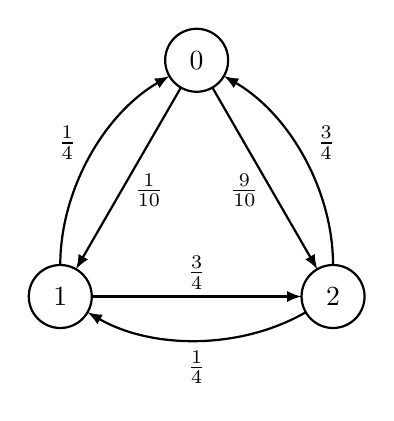
\begin{tikzpicture}[>=latex,thick]
\coordinate (A0) at (90:2);
\coordinate (A1) at (210:2);
\coordinate (A2) at (330:2);

\node at (A0) {$0$};
\node at (A1) {$1$};
\node at (A2) {$2$};

\draw (A0) circle[radius=0.4];
\draw (A1) circle[radius=0.4];
\draw (A2) circle[radius=0.4];

\draw[->,shorten >= 0.4cm,shorten <= 0.4cm] (A0) -- (A1);
\draw[->,shorten >= 0.4cm,shorten <= 0.4cm] (A0) -- (A2);
\draw[->,shorten >= 0.4cm,shorten <= 0.4cm] (A1) -- (A2);

\draw[->,shorten >= 0.4cm,shorten <= 0.4cm] (A1) to[out=90,in=-150] (A0);
\draw[->,shorten >= 0.4cm,shorten <= 0.4cm] (A2) to[out=90,in=-30] (A0);
\draw[->,shorten >= 0.4cm,shorten <= 0.4cm] (A2) to[out=-150,in=-30] (A1);

\def\R{1.9}
\def\r{0.7}

\node at (30:\r) {$\frac{9}{10}$};
\node at (150:\r) {$\frac1{10}$};
\node at (270:\r) {$\frac34$};

\node at (30:\R) {$\frac{3}{4}$};
\node at (150:\R) {$\frac1{4}$};
\node at (270:\R) {$\frac14$};

\end{tikzpicture}}
\end{center}
\end{block}
\end{column}
\begin{column}{0.48\textwidth}
\uncover<3->{%
\begin{block}{Markov-Kette $Y$}
Übergangsmatrix
\[
B=\begin{pmatrix}
0&\frac14&\frac34\\
\frac{1}{10}&0&\frac14\\
\frac{9}{10}&\frac34&0
\end{pmatrix}
\]
\vspace{-10pt}

\uncover<4->{%
Gewinnmatrix:
\vspace{-2pt}
\[
G=\begin{pmatrix*}[r]
0&-1&1\\
1&0&-1\\
-1&1&0
\end{pmatrix*}
\]}
\end{block}}
\vspace{-12pt}
\uncover<5->{%
\begin{block}{Gewinnerwartung}
\begin{align*}
&&&&
E(Y)
&=
U^t(G\odot B)p
\\
p&={\textstyle\frac13}U
&&\Rightarrow&
E(Y)&={\textstyle\frac1{15}}
\\
\overline{p}&={\tiny\frac{1}{13}\begin{pmatrix}5\\2\\6\end{pmatrix}}
&&\Rightarrow&
E(Y)&=0
\end{align*}
\end{block}}
\end{column}
\end{columns}
\end{frame}
\egroup
